\documentclass[10pt]{beamer}
% Class options include: notes, notesonly, handout, trans,
%                        hidesubsections, shadesubsections,
%                        inrow, blue, red, grey, brown

% Theme for beamer presentation.
\usepackage{beamerthemesplit} 
%\usepackage{times}
\usepackage{anysize}
\usepackage{fancyhdr}
\usepackage{graphicx}
\usepackage{pdfpages}
\usepackage{amsmath}
\usepackage{amssymb}
\usepackage{hyperref}
 \hypersetup{
 colorlinks=true,
 linkcolor=black
 }
% Other themes include: beamerthemebars, beamerthemelined, 
%                       beamerthemetree, beamerthemetreebars  

\title{\bfseries Term Indexing for the \\ Beagle Theorem Prover}    % Enter your title between curly braces
\author{Tim Cosgrove \vspace{-0.3cm}}                 % Enter your name between curly braces
\institute{COMP4006 Honours Research Project \\ \vspace{0.3cm}
Research School of Computer Science,\\
Australian National University \\ \vspace{0.3cm}
\texttt{u4843619@anu.edu.au} \\ \vspace{0.3cm}
Supervisor: Peter Baumgartner}      % Enter your institute name between curly braces
\date{\today}                    % Enter the date or \today between curly braces

\usetheme{PaloAlto}
\usecolortheme{crane}

\newcommand{\bcen}{\begin{center}}
\newcommand{\ecen}{\end{center}}

\begin{document}

% Creates title page of slide show using above information
\begin{frame}
  \titlepage
\end{frame}
\note{} % Add notes to yourself that will be displayed when
        % typeset with the notes or notesonly class options

\section[Outline]{}

% Creates table of contents slide incorporating
% all \section and \subsection commands
\begin{frame}
  \tableofcontents
\end{frame}

\section{The Beagle Theorem Prover}

\begin{frame}
  \frametitle{The Beagle Theorem Prover}   % Insert frame title between curly braces
  %Brief overview of beagle. Should include motivations for term-indexing (Pidgeon Hole problem
  \begin{itemize}
  \item<1-> First-Order-Logic resolution theorem prover with equality.
  \item<2-> Incorporates background theories, in particular integer arithmetic.
  \item<3-> Generates new clauses with a set of inference rules.
  \item<4-> Currently lacks an optimised method of locating clauses to use.
  \end{itemize}
\end{frame}

\section{Term Indexing} 

\begin{frame}
  \frametitle{Term Indexing Techniques}
  \begin{itemize}
  \item<1-> Terms consist of function symbols and variables: e.g. $f(a, x)$.
  \item<1-> Three important relations:
  \begin{itemize}
  \item<2-> 'Unifiable': $\sigma s = \sigma t$
  \item<2-> 'Instance Of': $s = \sigma t$
  \item<2-> 'Generalises': $\sigma s = t$
  \end{itemize}
  \item<3-> Top-Symbol Hashing.
  \item<3-> Discriminant Trees.
  \end{itemize}
  % Possibly just a results table. List and very briefly describe indexing
\end{frame}

\begin{frame}
  \frametitle{Fingerprint Indexing}
                  %Left Bot Right Top
  \begin{itemize}
  \item<1-> Maintain a collection of \emph{fingerprints} for terms.
  \item<2-> A term fingerprint is an array over $F \cup \{\mathbf{A, B, N}\}$.
  \item<3-> \includegraphics[page=6,scale=0.7,trim=5.5cm 20.5cm 5cm 4cm,clip]{schulz_fp-index_ext}
  \item<4-> {\footnotesize Schulz, Stephan: Fingerprint Indexing for Paramodulation and Rewriting. In:
  Lecture Notes in Computer Science volume 7364 pp. 447--483 (2012).}

  \end{itemize}
\end{frame}

\begin{frame}
  \frametitle{Fingerprint Indexing -- Example Fingerprint Index}
  % Structure of fingerprint indexes
                  %Left Bot Right Top
  \includegraphics[page=7,scale=0.7,trim=4cm 13.5cm 5cm 4.5cm,clip]{schulz_fp-index_ext}
\end{frame}


\begin{frame}
  \frametitle{Fingerprint Indexing -- Potential Performance}
  \begin{center}{\tiny
  \begin{tabular}{| l | r | r | r | r | r | r | r |} \hline
  Index & Run time & Sat time & PM time & PMI time & MGU time & BR time & BRI time \\ \hline
NoIdx & 16062.392 & 14078.300 &  8980.320 & 0.000 & 2545.080  & 2280.250 & 0.000\\
FP1 & 7006.758 & 6145.870 & 1816.100 & 25.710 & 450.760 & 379.570 & 40.150\\
FP6M & 6000.177 & 5385.810 & 1181.710 & 38.240 & 99.110 & 39.010 & 55.660\\
NPDT & 6082.246 & 5434.760 & 1184.750 & 64.910 & 83.110 & 33.200 & 79.910 \\\hline
  \end{tabular}}\vspace{0.5cm}
                  %Left Bot Right Top
  \includegraphics[page=13,scale=0.5,trim=6cm 8cm 7cm 12cm,clip]{schulz_fp-index_ext}
  \hspace{1cm}
                  %Left Bot Right Top
  \includegraphics[page=14,scale=0.5,trim=6cm 16.2cm 7cm 4cm,clip]{schulz_fp-index_ext}
  \end{center}
  % Results table from paper
\end{frame}

\section{Project Goals}

\begin{frame}
  \frametitle{Project Goals}
  \begin{itemize}
  \item<1-> Implement Fingerprint Term-indexing for Beagle.
  \begin{itemize}
  \item<1-> Involves modifying fingerprints to support background theories.
  \end{itemize}
  \item<2-> Experiment with indexing parameters for various problem sets
  \end{itemize}
\end{frame}

\end{document}
